\documentclass[aspectratio=169,unicode]{beamer}
\usepackage[ipa]{luatexja-preset}
\usepackage{url,luatexja-ruby}
\input{../temp/beamertemp}
\input{../temp/mylisting}
\setmainjfont{SourceHanSansJP}
\setmainfont{SourceHanSansJP}
\setmonofont{DroidSansMono}
\renewcommand{\familydefault}{\sfdefault}
\renewcommand{\kanjifamilydefault}{\gtdefault}
% \defaultfontfeatures{Ligature=TeX}
% \usebackgroundtemplate{
\includegraphics[width=.15\pagewidth]{sailormoonscript.png}}
\title{MoonScript Advent Calender}
\subtitle{3〜25日目}
\author{びしょ〜じょ}
\begin{document}
\maketitle
\section{自己紹介}
\begin{frame}
	こんにちは、びしょ〜j

	\pause
	% \bgroup\LARGE
	\bgroup\Huge
	\vspace{1\zw}
	これから\alert{\ruby{25日分のアドベントカレンダー}{\large{}闇のゲーム}}を

	\structure{5分}で進めるので自己紹介なんて時間かけられない。
	\vspace{1\zw}
	\egroup

	今日は12/02ということで\structure{2日目}から
\end{frame}
\section{2日目}
\begin{frame}[fragile]
	\frametitle{MoonScriptとは?}
	\begin{columns}
		\column[t]{.7\hsize}
		\begin{itemize}
			\item \alert{AltLua}で、PythonとかCoffeeScriptっぽい
			\item \lstinline|with|とか\structure{リスト内包表記}とか構文が増えている
			\item \lstinline|class|もあり、本格的な\structure{OOP}もできそう
		\end{itemize}
		\column[t]{.3\hsize}
		\begin{figure}[h]
			\vspace{-2\zw}\hspace{-5\zw}
\includegraphics[width=\columnwidth]{img/sailormoonscript.png}
		\end{figure}
	\end{columns}
	% \pause
	\begin{columns}
		\tiny
		\column[t]<2->{.4\hsize}
		\begin{lstlisting}[numbers=none,language=MoonScript,title=MoonScript class]
class Foo
	new: (@bar) =>
	baz: => print "bar: #{@bar}"
		\end{lstlisting}
		\uncover<3->{\hfill{}\structure{\normalsize{}compile! $\Rightarrow$}}

		\uncover<4->{
			{\LARGE{}\alert{かっこいい!! 短い!!}}

			オンラインコンパイラなどもあり手軽に始められる。詳しくは公式\footnote[frame]<4->{\url{http://moonscript.org}}をチェッキラッ
		}
		\column[t]<3->{.6\hsize}
		\begin{lstlisting}[numbers=none,language={[5.3]lua},title=generated Lua]
local Foo
do
  local _base_0 = {
    baz = function(self)
      return print("bar: " .. tostring(self.bar))
    end
  }
  _base_0.__index = _base_0
  local _class_0 = setmetatable({
    __init = function(self, bar)
      self.bar = bar
    end,
    __base = _base_0,
    __name = "Foo"
........
		\end{lstlisting}
	\end{columns}
\end{frame}
\section{3日目}
\begin{frame}[fragile]
	\frametitle{わ〜〜い12/03は冴草きいちゃんの誕生日だ!!!!!}
	\begin{columns}
	\scriptsize
		\column[b]{.41\hsize}
		\begin{lstlisting}[numbers=none,language=MoonScript]
require'luakatsu'
Aikatsu.Kii!
-- name    冴草 きい
-- actor   秋奈
-- birthday        12/03
-- blood_type      O
-- favorite_foods  ブレインサンダー
-- special_ablity  パソコン
-- favorite_brand  MAGICAL TOY
-- type    Pop
-- signature_songs マジカルタイム
-- sing    市倉 有菜
-- school  ドリーム・アカデミー
		\end{lstlisting}
		\column[b]<2->{.59\hsize}
		\begin{lstlisting}[numbers=none,language=MoonScript,title=\alert{Luakatsu v3 draft function}]
require'luakatsu'
-- `find_birthday` returns matched idol table
((x) -> x and x!) Aikatsu.find_birthday"12/03"
-- name    冴草 きい
-- actor   秋奈
-- birthday        12/03
-- blood_type      O
-- favorite_foods  ブレインサンダー
-- special_ablity  パソコン
-- favorite_brand  MAGICAL TOY
-- type    Pop
-- signature_songs マジカルタイム
-- sing    市倉 有菜
-- school  ドリーム・アカデミー
		\end{lstlisting}
	\end{columns}
おめでとう! 秋奈さんもガルパン劇場版おめでとうございます!!!!

\pause
!!Luakatsu v3も\alert{12/03リリース}予定!!
\end{frame}
\section{4日目}
\begin{frame}[fragile]
	\frametitle{リスト内包表記}
	\bgroup\scriptsize
	\begin{lstlisting}[numbers=none,language=MoonScript]
t1 = {i for i = 1, 5}
-- {1, 2, 3, 4, 5}
t2 = {i for i = 1, 10 when i % 2 == 0}
-- {2, 4, 6, 8, 10}
t3 = {k, v * 3 for k, v in pairs{x:1, y:2, z:3}}
-- {x:3, y:6, z:9}
	\end{lstlisting}
	\egroup

	これを用いてテーブルのdeep-copyも簡単にできる。
	\bgroup\scriptsize
	\begin{lstlisting}[numbers=none,language=MoonScript]
dc = (t) ->
	{k, (type(v) == "table" and (dc v) or v) for k, v in pairs t}
t = x: 1, y: 2, z: 3
t_ = dc t
t_.m = 4
print t.m -- nil
print t_.m -- 4
	\end{lstlisting}
	\egroup

\end{frame}
\section{5日目}
\begin{frame}[fragile]
	\frametitle{REPLがある\footnote[frame]{\url{https://github.com/Nymphium/moor}}}

	MoonScriptの作者leafo氏がちょろっとかいたREPLを改良したものを改良した。

	一部オートインデントや、inspectモジュール\footnote[frame]{\url{https://github.com/kikito/inspect.lua}}など使い勝手がよくなっているよ!
	\scriptsize
	\begin{lstlisting}[numbers=none]
$ moor -h
Usage: moonr [options]

   -h         print this message
   -n         continue running REPL after "e" option completed
   -e STR     execute string as MoonScript code
   -l LIB     load library before run REPL
   -L LIB     execute `LIB = require"LIB"` before run REPL

$ moor
moor on MoonScript version 0.3.2 on Lua 5.3
> string.split_t = (dlm) =>
?  str = self\match"#{dlm}$" and self or self .. dlm
?  [p for p in str\gmatch "(.-)#{dlm}"]
?
> "渋谷凛,島村卯月,本田未央"\split_t ","
{ "渋谷凛", "島村卯月", "本田未央" }
	\end{lstlisting}
\end{frame}
\section{6日目}
\begin{frame}[fragile]
	\frametitle{analyzer for MoonScript}

	みなさんは\alert{Vim}を使っている可能性が高いと思いますが、Syntastic\footnote[frame]{強力なシンタックスチェッカープラグイン。\url{https://github.com/scrooloose/syntastic}}%
	にMoonScriptのアナライザを書いた\footnote[frame]{\url{http://github.com/nymphium/syntastic-moonscript}}。

	$\bullet$しくみ
	\uncover<2->{
		\bgroup\small
		\begin{enumerate}
			\item ソースをLuaにコンパイル
			\item Luacheck\footnote[frame]{\url{http://luacheck.readthedocs.org}}を通す
			\item \lstinline|moonc -X src.moon|でソースと生成されたLuaの行、エラー行を照らし合わせる

				(ここアホっぽい)
		\end{enumerate}
		\egroup
	}

	$\bullet$実装

	\begin{columns}
		\column[t]<3->{.2\hsize}
		\fbox{昔: シェルスクリプト}
		\column[t]<3->{.2\hsize}
		\vspace{-2\zw}
		\begin{center}
		$\Rightarrow$

		\uncover<5->{\alert{10倍速}
	
		{\tiny{}(もともとがしょぼかった)}}
		\end{center}
		\column[t]<4->{.2\hsize}
		\fbox{今: \structure{MoonScript}}
	\end{columns}
\end{frame}

\section{7日目}
\begin{frame}[fragile]
\frametitle{クラス}
\begin{columns}
	\column[t]{.5\hsize}
	\begin{lstlisting}[numbers=none,language=MoonScript]
class Cls
	new: (...) =>
		for i in *{...}
			table.insert @, i
	__add: (l, r) ->
		#l + #r
	__sub: (l, r) ->
		#l - #r

i1 = Cls 1, 2, 3, 4, 5
i2 = Cls 6, 7, 8

print i1 - i2 -- 2
	\end{lstlisting}
	\column[t]{.5\hsize}
	\begin{itemize}
		\item 内部的にはテーブルにメタテーブルを突っ込む感じになる。
		\item \lstinline|new|メソッドがコンストラクタになる。
	\end{itemize}
\end{columns}
\end{frame}
\section{8日目}
\begin{frame}[fragile]
	\frametitle{\lstinline|with|構文}
	\begin{columns}
		\footnotesize
		\column[t]{.49\hsize}
		\begin{lstlisting}[numbers=none,language=MoonScript]
foo = (t) ->
	i = {}

	if type(t) == "table"
		for p in *t
			table.insert i, p
	else
		setmetatable i, {t}
	
	i -- return value
		\end{lstlisting}
		\pause
		\column[t]{.01\hsize}
		\vfill
		\structure{\normalsize{}$\Rightarrow$}
		\column[t]{.49\hsize}
		\begin{lstlisting}[numbers=none,language=MoonScript]
foo_with = (t) ->
	with i = {}
		if type(t) == "table"
			for p in *t
				table.insert i, p
		else
			setmetatable i, {t}
		\end{lstlisting}
	\end{columns}
	\vspace{2\zw}

	チャンク中に変数名をバインドし、そのチャンクの戻り値とする。
\end{frame}
\section{9日目}
\begin{frame}[fragile]
	\frametitle{{\rm{}Lua\LaTeX{}}でもMoonScript}
	\begin{columns}
		\column[t]{.4\hsize}
		\tiny
		\begin{lstlisting}[numbers=none=LaTeX]
...
\usepackage{luacode}
\directlua{
	require 'lualoader'
	ms = require'moonscript.base'

	function directmoon(str)
		return (ms.loadstring(str))()
	end
}
...
\begin{luacode*}
-- オフサイドルールに気をつける
local ok, cont = pcall(directmoon,[[
for i = 1, 10
	tex.print i

tex.print "coinsLT #11"\match"(%S+)"
]])

if ok then
	tex.print("\\\\イェ〜イ")
else
	tex.print("error: ", cont)
end
\end{luacode*}
		\end{lstlisting}
		\column[t]{.6\hsize}

\alert{実行結果:}

\begin{luacode*}
local ok, cont = pcall(directmoon, [[
for i = 1, 10
	tex.print i

tex.print "coinsLT #11"\match"(%S+)"
]])

if ok then
	tex.print("\\\\イェ〜イ")
else
	tex.print("error: ", cont)
end
\end{luacode*}

\vspace{2\zw}
	非常に雑なのでいろいろ問題はある{\scriptsize{}(\lstinline|luacode*|環境じゃないとバックスラッシュなどが使えないし、逆に\lstinline|luacode*|環境だと{\rm\LaTeX{}}コマンドが簡単には使えない、等)}。
	\end{columns}
\end{frame}
\section{10日目}
\begin{frame}[fragile]
	\frametitle{なにで書く? \textcircled{1}}
	\alert{Vimでもいいんだけど}

	オープンソースなLua IDEであるZeroBrane Studio\footnote[frame]{\url{http://studio.zerobrane.com/}}%
	にはMoonScript用プラグイン\footnote[frame]{\url{https://github.com/pkulchenko/ZeroBranePackage/blob/master/moonscript.lua/}}があり、導入することでMoonScriptもバンバン書ける。
	不安定なのでバンバン落ちる。
	\begin{columns}
		\column[t]{.5\hsize}
		\tiny
		\begin{lstlisting}[numbers=none,language={[5.3]lua}]
editor.fontname = "Monaco"
editor.fontsize = 13
acandtip.droprest = true
acandtip.nodynwords = true
acandtip.startat = 2
acandtip.startegy = 2
autocomplete = true
		\end{lstlisting}
		\column[t]{.5\hsize}
		\begin{figure}[h]
			\centering
			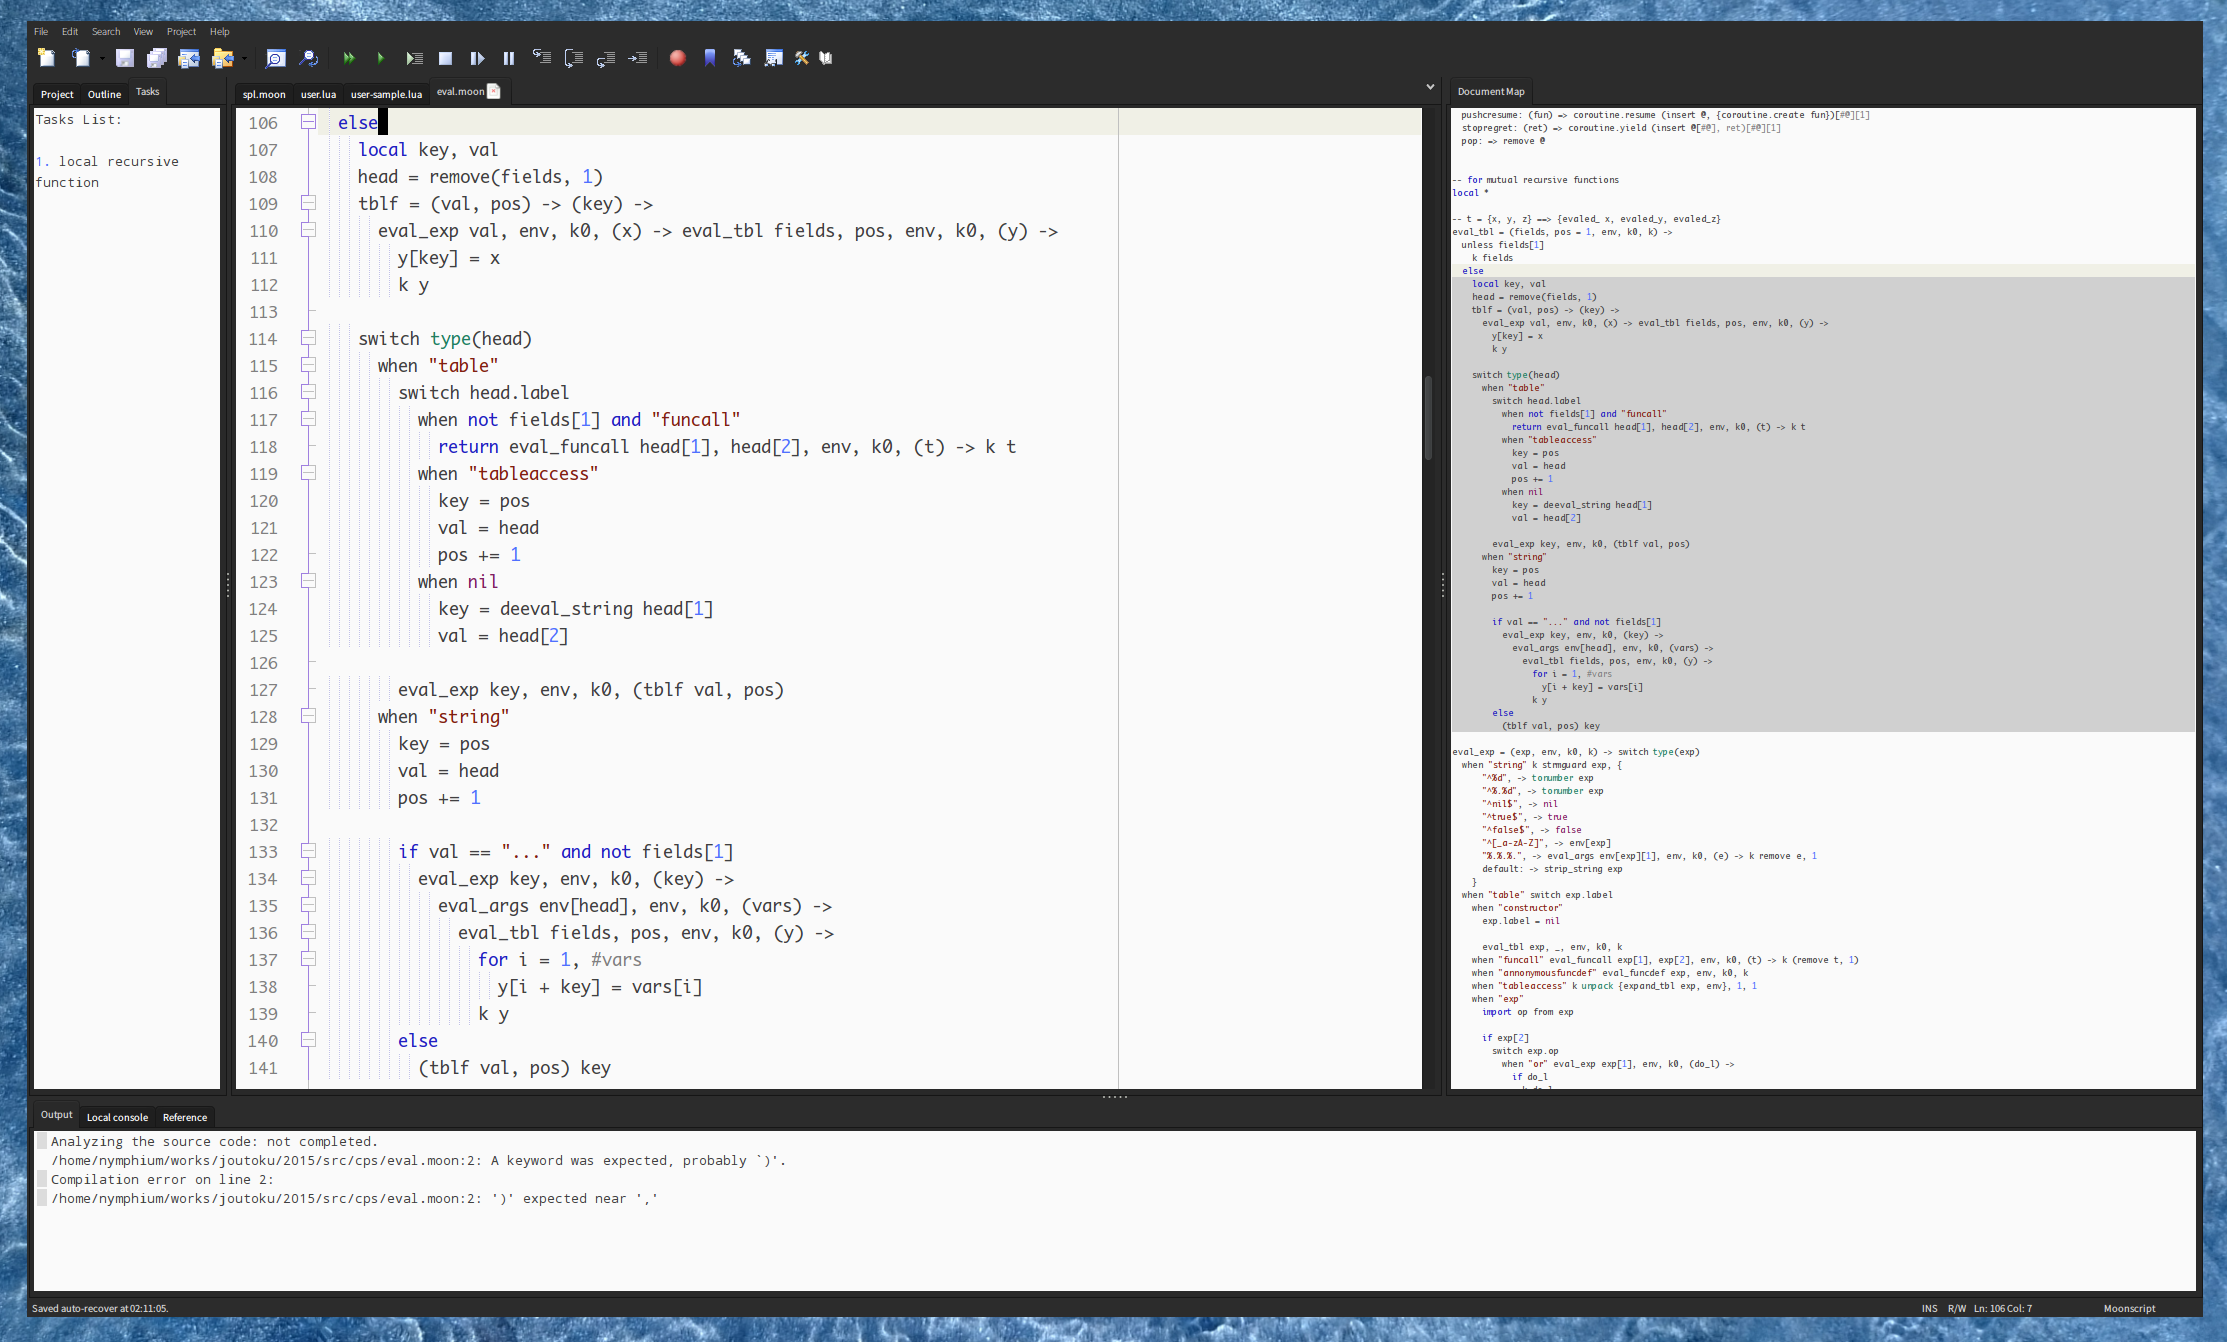
\includegraphics[width=\columnwidth]{img/zbstudio.png}
		\end{figure}
	\end{columns}
\end{frame}

\section{11日目}
\begin{frame}[fragile]
	\frametitle{なにで書く? \textcircled{2}}
	\alert{Vimでもいいんだけど}

	Howl Editor\footnote[frame]{\url{http://howl.io/}}はMoonScriptで拡張が書ける! MoonScriptも書ける! 一石二鳥!!

	\begin{columns}	
		\column[t]{.5\hsize}
		\tiny
		\begin{lstlisting}[numbers=none,language=MoonScript]
import config from howl


config.hungry_completion = true

howl.bindings.push {
	editor:
		shift_alt_c: 'editor-toggle-comment'
	ctrl_f: 'open'
	alt_e: 'cursor-word-right'
	alt_w: 'cursor-word-left'
	alt_s: 'save'
	ctrl_w:
		ctrl_w: 'quit'
	r:      'editor-redo'
	u:      'editor-undo'
}

howl.command.vi_on!
	\end{lstlisting}
	\column[t]{.5\hsize}
	\begin{figure}[h]
		\centering
		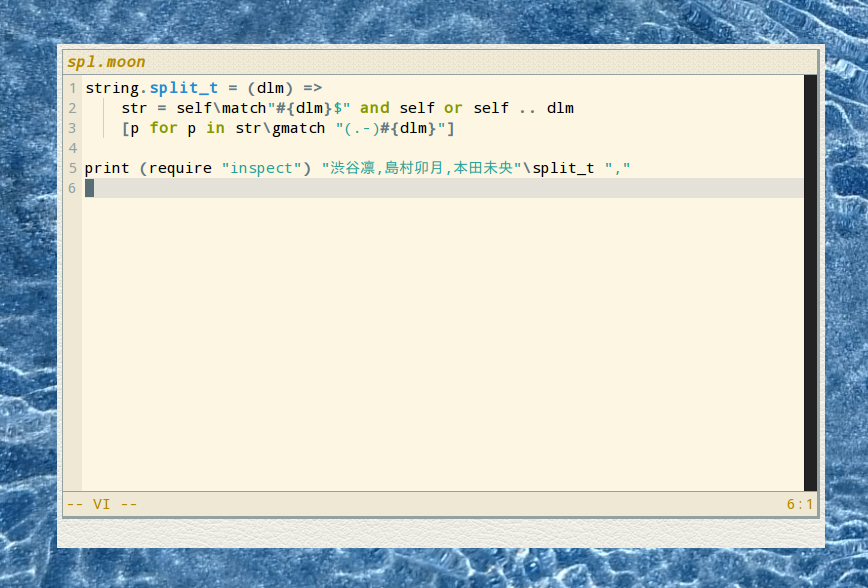
\includegraphics[width=\columnwidth]{img/howl.png}
		\end{figure}
	\end{columns}
\end{frame}
\section{12日目}
\begin{frame}[fragile]
	\frametitle{MoonScript-Luaのバージョン問題}
	MoonScriptはLua5.1ベースで開発されており\footnote[frame]{2015 12/02(commit ae2558ab67d8227b870cee1597a608c98727a924)現在}、パーサーもLua5.1までしか対応していない。

	でもLua5.3上でMoonScriptはうごくので\vspace{2\zw}

	\begin{columns}
		\scriptsize
		\newcommand{\lv}[1]{{\tiny{}(v{#1}〜)}}
		\column[t]{.5\hsize}
		\alert{これできる}
		\begin{itemize}
			\item \lstinline|__len|メタメソッド\lv{5.2}
			\item \lstinline|bit32|モジュール\lv{5.2}
			\item \lstinline|utf8|モジュール\lv{5.3}
		\end{itemize}
		\column[t]{.5\hsize}
		\alert{これできない}
		\begin{itemize}
			\item \lstinline|>>|、\lstinline|<<|演算子\lv{5.3}
			\item \lstinline|__shl|、\lstinline|__shr|メタメソッド\lv{5.3}\footnote[frame]{metatableに登録はできるが、対応する演算子が使えないため。}
			\item \lstinline;|;、\lstinline|&|演算子\lv{5.3}
			\item \lstinline|__bor|、\lstinline|__band|メタメソッド\lv{5.3}\footnotemark[10]
			\item \lstinline|//|演算子\lv{5.3}
			\item \lstinline|__idiv|メタメソッド\lv{5.3}\footnotemark[10]
			\item \lstinline|~|演算子\lv{5.3}
		\end{itemize}
	\end{columns}
\end{frame}
\begin{frame}[fragile]
	\frametitle{どうしても使いたいときは…}
	\begin{itemize}
		\begin{columns}
			\column[t]{.5\hsize}
			\item \lstinline|load|つかおう!\footnote[frame]{文字列にして\lstinline|load|につっこむため、tableそのままマズいのでサンプルでは変数名を文字列として渡している。}
				\bgroup\tiny
				\begin{lstlisting}[numbers=none,language=MoonScript]
strbin = (l, r, op) ->
	load("return #{l} #{op} #{r}")!

print(strbin(1, 10, "<<")) -- 1024

class T
	__shl: (r) =>
		table.insert @, r

t = T!
strbin "t", 3, "<<"
print(t[1]) -- 3
				\end{lstlisting}
				\egroup

			\column[t]{.5\hsize}
			\item \lstinline|require|つかおう!

				\lstinline|require|で\structure{luaファイルを}読みこめばLua処理系が処理してくれるのでOK\footnote[frame]{もちろんmoonファイルはまずMoonScriptが処理するのでパースに失敗する。}。

				\bgroup\tiny
				\begin{lstlisting}[numbers=none,language={[5.3]lua}]
-- shl.lua, callee
return 1 << 10
				\end{lstlisting}
				\begin{lstlisting}[numbers=none,language=MoonScript]
-- moon file, caller
print require 'shl' -- 1024
				\end{lstlisting}
				\egroup
		\end{columns}
	\end{itemize}
\end{frame}

\input{13_18}
\input{19_25}
\end{document}
